\chapter{Conclusion}\label{ch:conclusion}

\section{Synthetic Samples}
  Because we couldn't get any visible or audible results with our filtering method of real recordings with two 
microphones and one sound source and it was even worse with two sound sources at the same time, we have 
decided to try recording each person separately, using one microphone and then synthetically articulate data, 
as if we recorded two sound sources at the same time to two microphones by adding delay and gain on both 
sources which made it look and sound realistically.\\
  In order to create samples to sound as realistic as possible we had to look in delay differences as well as 
gain loss over distance. \\


  Using synthetic samples also gives us more flexibility when testing the code, we just need to adjust the 
angle that we want to place sources at. 
  \subsection{Code}
  Code for making synthetic samples needs angles that we want to place sources at and the gap between the 
microphones. Then we can use code we did for calculating shift in delays from a given angle. Shift the signal 
by samples, calculated and add gain ratio. \\
  Relationship of sound strength is what we call gain ratio. Sound strength falls by a ratio of \( \frac{1}{2}
\) when the distance is doubled. Which means that sound strength follows distance inverse-proportionally. 
  By giving one of the microphones gain ratio of 1 we can calculate what is the ratio for the other 
microphone. Figure \ref{fig:ratioDependence} illustrates the variables used in the equations.
\begin{figure}[htp]
	\centering
	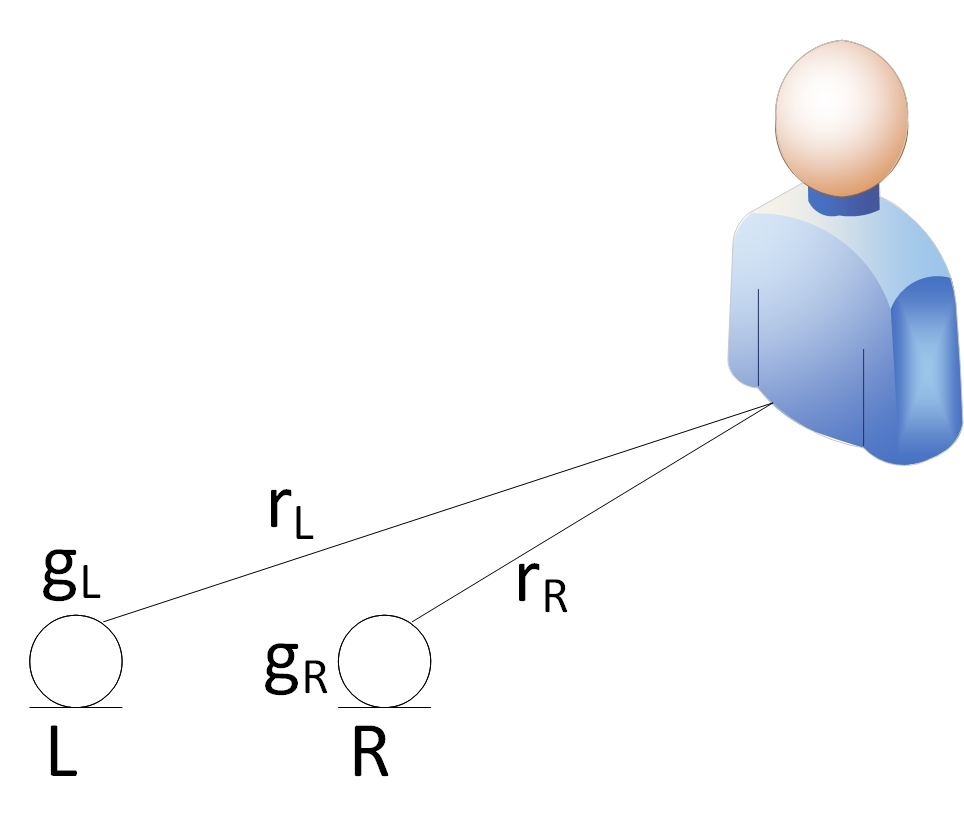
\includegraphics[width=0.35\textwidth]{Illustrations/gainRatio.jpg}
	\caption{Gain ratio dependence on distance}
	\label{fig:ratioDependence}
\end{figure}
\todo {check matlab script, see if left and right are correctly }
 \[\frac{g_L}{g_R} = \frac{r_R}{r_L} \]\\
Using this proportion and keeping \(g_L\) as 1 we can calculate gain \(g_R\), which we will multiply with 
right microphone data to get realistic gain loss. Distances \(r_L\) and \(r_R\) here are the same distances, 
which we calculate in delay code. This means that in order to get the gain ratio for right microphone we just 
need to divide distance to the left microphone (\(r_L\)) by distance to the right microphone (\(r_R\)).